\chapter{Architectural Views}

\section{Context View}

\subsection{Stakeholders' uses of this view}

There are three main stakeholders of the system: the volunteers, victims, developers. \\

The volunteers use this view to understand how they will help the victims by sharing information with website.
The victims use this view to understand how they can get help to get food, healthcare, etc.
The developers use this view to understand how they can build a bridge between victims and volunteers and how they can achieve to forward the validated information as fast as possible.

\subsection{Context Diagram}

\begin{figure}[H]
    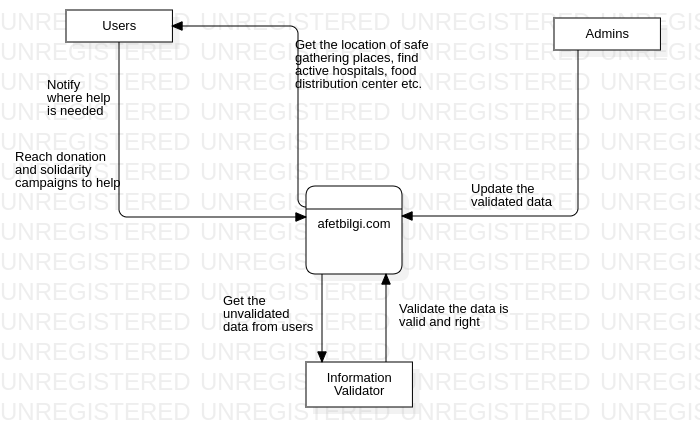
\includegraphics[scale = 0.6]{assets/Context Diagram.png}
    \caption[Context Diagram for afetbilgi.com]{Context Diagram for afetbilgi.com}
\end{figure}

As it can be observed from the context diagram, the system interacts with 3 external entities. These are users, admins and information validators. Afetbilgi.com users can use this website for 2 purpose. It can be used to deliver help or it can be used to get help who are affected by the disaster.
in addition to that, information validator gets the all information which delivered to them and by reaching the authorities validates the information. In meanwhile, admins update the database with these validated datas in the system. 

\subsection{External Interfaces}

In this section, the external interfaces of the afetbilgi.com will be provided.

\begin{figure}[H]
    
\includegraphics[scale = 0.4]{assets/externalInterfaces.png}
    \caption[External Interfaces Class Diagram for Afetbilgi]{External Interfaces Class Diagram for Afetbilgi}
\end{figure}

\begin{center}
    \begin{table}[H]
        \begin{tabular}{| m{6cm}| m{8cm} |}
            \hline
            \textbf{Operation} & \textbf{Description} \\
            \hline
            generatePdf & The website generate the pdf which contains the selected city crucial information in compact form as a downloadable file by users.\\
            \hline
            showLocationsOnMaps & Website shows the important locations on the map.\\
            \hline
            changeLanguage & Users can choose a language between Turkish, English, Kurdi and Arabic.\\
            \hline
            selectCity & Website filter the datas according to selected city.\\
            \hline
            showInformations & Shows the information as subparts on the website mainpage.\\
            \hline
            editCode & Developers can edit the code in the source files.\\
            \hline
            updateDatabase & Developers can update the database with the validated information.\\
            \hline
            getData & Users can reach the validated data by using this website.\\
            \hline
            sendEmail & In case of truth of information or error in server, users can send an email.\\
            \hline
            pushRequest & Developers can push the code changes to Github Repository.\\
            \hline
            pullRequest & Developers can pull the code from the Github Repository.\\
            \hline
            clone & Developers can download the code from the Github Repository.\\
            \hline
            commit & Developers can record changes in their code.\\
            \hline
            log & Developers can look at it previous commits.\\
            \hline
            getClickableIcons & Google Maps API gets the icons such as hospital and pharmacies to show on map.\\
            \hline
        \end{tabular}
        \caption[External Interface Operation Descriptions]{External Interface Operation Descriptions}
    \end{table}
\end{center}

\subsection{Interaction scenarios}

\begin{figure}[H]
    
\includegraphics[scale = 0.5]{assets/Activity DiagramMaps.png}
    \caption[Activity Diagram for Google Maps API Afetbilgi Interactions]{Activity Diagram for Google Maps API Afetbilgi Interactions}
\end{figure}

\begin{figure}[H]
    
\includegraphics[scale = 0.5]{assets/Activity DiagramEditingCode.png}
    \caption[Activity Diagram for Developer and Github Editing Code Interactions]{Activity Diagram for Developer and Github Editing Code Interactions}
\end{figure}

\section{Functional View}

\subsection{Stakeholders' use of this view}

There are three main stakeholders of the system: the volunteers, victims and developers. \\

The volunteers use this view to find locations which can help to go there or donating money.
The victims especially use this view to make use of Google Maps API since it is very helpful to find all crucial locations in a compact form near them.
The developers use this view to add new functionalities to this system so that they can reach more people and help to faster delivery of aid.

\subsection{Component Diagram}

\begin{figure}[H]
    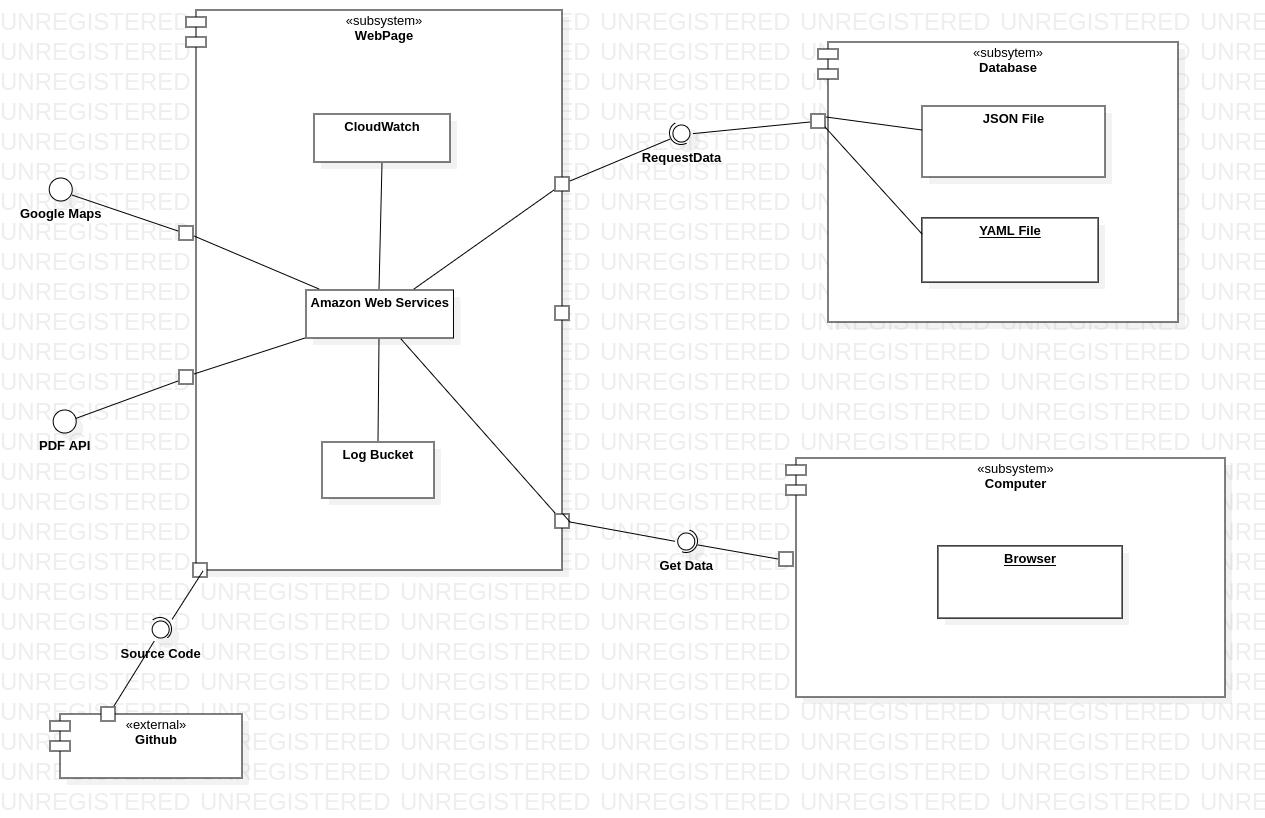
\includegraphics[scale = 0.4]{assets/ComponentDiagram.png}
    \caption[Component Diagram for Afetbilgi]{Component Diagram for Afetbilgi}
\end{figure}
~\\~\\
Afetbilgi.com has three main subsystem which are Amazon Web Services, Database and Computer.

\begin{itemize}
    \item Web Service consists of three parts, Amazon Web Services, CloudWatch and LogBucket.
    \item Computer has a part which is browser. It allows to search in internet and gets the information with a graphical userface.
    \item When the user reach the webpage via browser, comptuer sends a request to the web services. Webservice holds their database in a two different file type. It requests these files and parser them to send the information to the users. 
    \item Database uses two different file type which are JSON file and YAML file.
    \item GitHub is an external component which stores the source code of the system. Moreover, when the developers make a change in their system, it allows them to update the whole webservice by Github. 
    \item When the users try to do tasks which uses Google Maps API or PDF API, webservice interacts with these APIs to created necessary information for the user.
    \item The interface between the computer and webservice uses a https protocol to communication. HTTPS is encrypted in order to increase security of data transfer.
\end{itemize}

\subsection{Internal Interfaces}

In this section, the internal interfaces of afetbilgi will be provided. \\

\begin{figure}[H]
    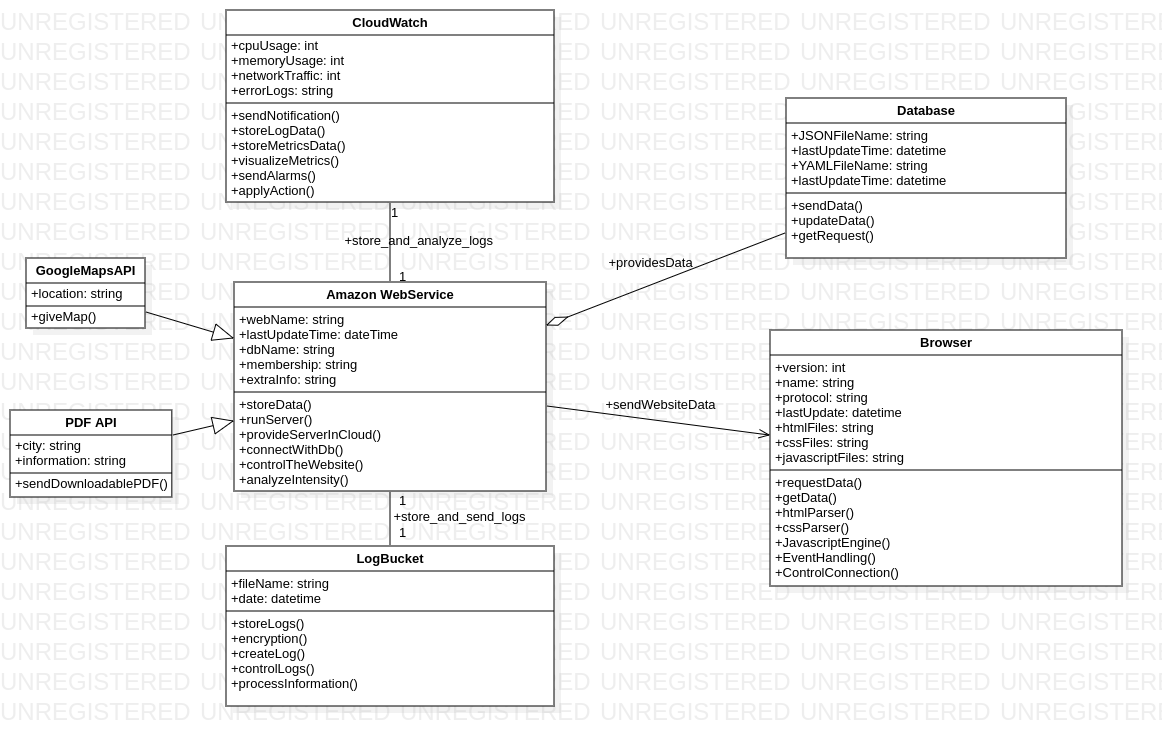
\includegraphics[scale = 0.4]{assets/InternalInterfaces.png}
    \caption[Internal Interface of Afetbilgi]{Internal Interface of Afetbilgi}
\end{figure}

\subsection{Interaction Patterns}

As shown in Figure 4.6, the internal interfaces of Afetbilgi are Amazon Web Service, CloudWatch, LogBucket, Database and Browser. The operations of interfaces can be described in below. \\

\begin{itemize}
    \item There are two different API which is implemented into to webservice. According to users' needs the necessary API used to create the PDF file which contains information or shows the important locations on Google Maps.
    \item There are two internal interface which has an association with the Amazon Web Service which are CloudWatch and LogBucket. With these internal interfaces, it stores the log of website and give an opportunity of analyzing the metrics of website.
    \item Database which is an internal interface allow website 
\end{itemize}

\section{Information View}

\subsection{Stakeholders' uses of this view}

\subsection{Database Class Diagram}

\subsection{Operations on Data}

\section{Deployment View}

\subsection{Stakeholders' uses of this view}

\subsection{Deployment Diagram}

\section{Design Rationale}